\documentclass[notes,11pt, aspectratio=169]{beamer}

\usepackage{pgfpages}
% These slides also contain speaker notes. You can print just the slides,
% just the notes, or both, depending on the setting below. Comment out the want
% you want.
\setbeameroption{hide notes} % Only slide
%\setbeameroption{show only notes} % Only notes
%\setbeameroption{show notes on second screen=right} % Both

%\usepackage[scaled=1.0]{helvet}
\usepackage{array}


\usepackage{tikz}
\usepackage{verbatim}
\setbeamertemplate{note page}{\pagecolor{gray!5}\insertnote}
\usetikzlibrary{positioning}
\usetikzlibrary{snakes}
\usetikzlibrary{calc}
\usetikzlibrary{arrows}
\usetikzlibrary{decorations.markings}
\usetikzlibrary{shapes.misc}
\usetikzlibrary{matrix,shapes,arrows,fit,tikzmark}
\usepackage{amsmath}
\usepackage{mathpazo}
\usepackage{hyperref}
\usepackage{lipsum}
\usepackage{multimedia}
\usepackage{graphicx}
\usepackage{multirow}
\usepackage{graphicx}
\usepackage{dcolumn}
\usepackage{bbm}
\newcolumntype{d}[0]{D{.}{.}{5}}

\usepackage{changepage}
\usepackage{appendixnumberbeamer}
\newcommand{\beginbackup}{
   \newcounter{framenumbervorappendix}
   \setcounter{framenumbervorappendix}{\value{framenumber}}
   \setbeamertemplate{footline}
   {
     \leavevmode%
     \hline
     box{%
       \begin{beamercolorbox}[wd=\paperwidth,ht=2.25ex,dp=1ex,right]{footlinecolor}%
%         \insertframenumber  \hspace*{2ex} 
       \end{beamercolorbox}}%
     \vskip0pt%
   }
 }
\newcommand{\backupend}{
   \addtocounter{framenumbervorappendix}{-\value{framenumber}}
   \addtocounter{framenumber}{\value{framenumbervorappendix}} 
}


\usepackage{graphicx}
\usepackage[space]{grffile}
\usepackage{booktabs}

% These are my colors -- there are many like them, but these ones are mine.
\definecolor{blue}{RGB}{0,114,178}
\definecolor{red}{RGB}{213,94,0}
\definecolor{yellow}{RGB}{240,228,66}
\definecolor{green}{RGB}{0,158,115}

\hypersetup{
  colorlinks=false,
  linkbordercolor = {white},
  linkcolor = {blue}
}


%% I use a beige off white for my background
\definecolor{MyBackground}{RGB}{255,253,218}

%% Uncomment this if you want to change the background color to something else
%\setbeamercolor{background canvas}{bg=MyBackground}

%% Change the bg color to adjust your transition slide background color!
\newenvironment{transitionframe}{
  \setbeamercolor{background canvas}{bg=white}
  \begin{frame}}{
    \end{frame}
}

\setbeamercolor{frametitle}{fg=blue}
\setbeamercolor{title}{fg=black}
\setbeamertemplate{footline}[frame number]
\setbeamertemplate{navigation symbols}{} 
\setbeamertemplate{itemize items}{-}
\setbeamercolor{itemize item}{fg=blue}
\setbeamercolor{itemize subitem}{fg=blue}
\setbeamercolor{enumerate item}{fg=blue}
\setbeamercolor{enumerate subitem}{fg=blue}
\setbeamercolor{button}{bg=MyBackground,fg=blue,}

%%% TIKZ STUFF
\tikzset{   
	every picture/.style={remember picture,baseline},
	every node/.style={anchor=base,align=center,outer sep=1.5pt},
	every path/.style={thick},
}
\newcommand\marktopleft[1]{%
	\tikz[overlay,remember picture] 
	\node (marker-#1-a) at (-.3em,.3em) {};%
}
\newcommand\markbottomright[2]{%
	\tikz[overlay,remember picture] 
	\node (marker-#1-b) at (0em,0em) {};%
}
\tikzstyle{every picture}+=[remember picture] 
\tikzstyle{mybox} =[draw=black, very thick, rectangle, inner sep=10pt, inner ysep=20pt]
\tikzstyle{fancytitle} =[draw=black,fill=red, text=white]
%%%% END TIKZ STUFF


% If you like road maps, rather than having clutter at the top, have a roadmap show up at the end of each section 
% (and after your introduction)
% Uncomment this is if you want the roadmap!
% \AtBeginSection[]
% {
%    \begin{frame}
%        \frametitle{Roadmap of Talk}
%        \tableofcontents[currentsection]
%    \end{frame}
% }
\setbeamercolor{section in toc}{fg=blue}
\setbeamercolor{subsection in toc}{fg=red}
\setbeamersize{text margin left=1em,text margin right=1em} 

\newenvironment{wideitemize}{\itemize\addtolength{\itemsep}{10pt}}{\enditemize}
\newenvironment{wideenumerate}{\enumerate\addtolength{\itemsep}{10pt}}{\endenumerate}

\usepackage{environ}
\NewEnviron{videoframe}[1]{
  \begin{frame}
    \vspace{-8pt}
    \begin{columns}[onlytextwidth, T] % align columns
      \begin{column}{.58\textwidth}
        \begin{minipage}[t][\textheight][t]
          {\dimexpr\textwidth}
          \vspace{8pt}
          \hspace{4pt} {\Large \sc \textcolor{blue}{#1}}
          \vspace{8pt}
          
          \BODY
        \end{minipage}
      \end{column}%
      \hfill%
      \begin{column}{.42\textwidth}
        \colorbox{green!20}{\begin{minipage}[t][1.2\textheight][t]
            {\dimexpr\textwidth}
            Face goes here
          \end{minipage}}
      \end{column}%
    \end{columns}
  \end{frame}
}

\title[]{\textcolor{blue}{ECN 453: Pricing and Price Discrimination 3}}
\author[PGP]{}
\institute[FRBNY]{\small{\begin{tabular}{c c c}
Nicholas Vreugdenhil \\
\end{tabular}}}
\date{} 

\begin{document}

% Title Slide
\begin{frame}
\maketitle
  \centering
\end{frame}

% INTRO

\begin{frame}{Plan}
	\begin{wideenumerate}
		\item Non-linear pricing
		\item Should price discrimination be legal?
	\end{wideenumerate}
\end{frame}

\begin{frame}{Plan}
	\begin{wideenumerate}
		\item \textbf{Non-linear pricing}
		\item Should price discrimination be legal?
	\end{wideenumerate}
\end{frame}

\begin{frame}{Non-linear pricing}
\begin{columns}
	\begin{column}{0.6\textwidth}
		\begin{wideitemize}
			\item Consumers often decide not just \textit{whether} to buy a produce but also \textit{how much}.
			\item \textbf{Examples}
			\begin{wideitemize}
				\item How many scoops of ice-cream?
				\item How much electricity/water/gas to use?
			\end{wideitemize}
			\item \textbf{Non-linear pricing}: when the price changes with the total quantity purchased.
			\begin{wideitemize}
				%\item As we will see, this is another example of `price discrimination by self-selection', but following the book I present it in its own section.
				\item e.g. first ice-cream scoop costs \$5, second costs \$2, third \$1,...
			\end{wideitemize}
		\end{wideitemize}
	\end{column}
	\begin{column}{0.4\textwidth}
	\begin{figure}
		\includegraphics[scale=0.15]{icecream.jpeg}
		\caption{Getty Images}
	\end{figure}
	\end{column}
\end{columns}
\end{frame}

\begin{frame}{Non-linear pricing}
	\begin{wideitemize}
		\item We will look at a particular form of non-linear pricing: \textbf{two-part tariffs} 
		\begin{wideitemize}
			\item We will begin by studying the case with homogeneous consumers (i.e. identical consumers who all have the same demand curve). 
		\end{wideitemize}
		\item A two-part tariff is in the form: 
		\begin{align*}
			\text{two-part tariff = }f + pq
		\end{align*}
		%\item Where:
		\begin{wideitemize}
			\item $f$: fixed part (e.g. golf club membership)
			\item $p$: variable part (e.g. greens fee you pay every time you play golf)
			\item $q$: quantity
		\end{wideitemize}
		\item The \textbf{price per unit} (i.e. average price) is $p+f/q$ and decreases as quantity $q$ increases.
		\item We will see how a two-part tariff can be more profitable for a seller than a single price.
	\end{wideitemize}
\end{frame}

\begin{frame}{Non-linear pricing: how should the seller choose $f$ and $p$?}
	\begin{columns}
		\begin{column}{0.5\textwidth}
			\begin{figure}
			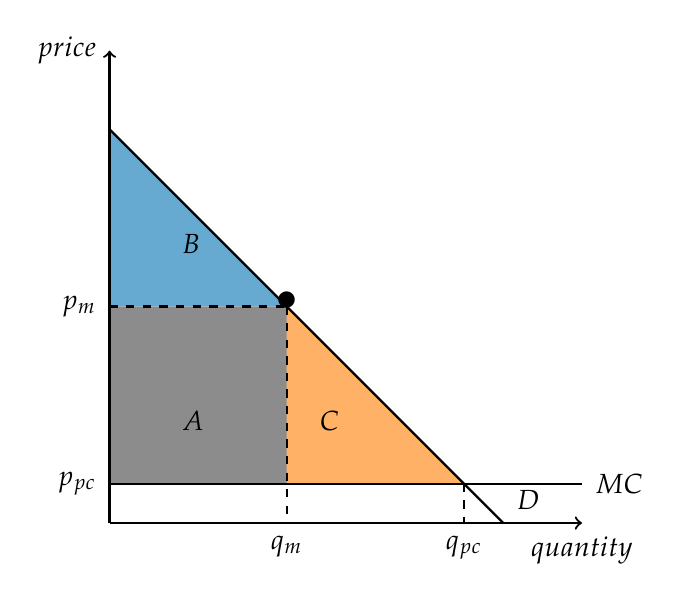
\begin{tikzpicture}[scale=0.5]
				\fill [darkgray!60] (0,1) -- (0,5.5) -- (4.5,5.5) -- (5.5,1) -- cycle;
				\fill [blue!60] (0,5.5) -- (4.5,5.5) -- (0,10) -- cycle;
				\fill [orange!60] (4.5,1) -- (4.5,5.5) -- (9,1) -- cycle;
				
				%y axis.....................
				\draw [->] (0,0) to (0,12) node [left] {$price$};
				
				%x axis......................
				\draw [->] (0,0) to (12,0) node [below] {$quantity$};
				
				% D curve...................
				\draw [thick] (0,10)  to  (10,0)  node [above right] {$D$};
				
				% MR curve....................
				%\draw [thick] (0,10) to (5,0);
				%\node [above right] at (4.5,-0.1) {$MR$};
				
				% MC=S curve...................
				\draw [thick] (0,1)  to  (12,1)  node [right] {$MC$};
				
				% dashed lines to equilibrium.............
				\draw [dashed] (0,5.5) node [left] {$p_m$} to (4.55,5.5); 
				\draw [dashed] (4.5,5.5) to (4.5,0) node [below] {$q_m$};
				
				% dashed lines to new equilibrium.........
				\draw [dashed] (0,1) node [left] {$p_{pc}$} to (9,1); 
				\draw [dashed] (9,1) to (9,0) node [below] {$q_{pc}$};
				
				% equilibrium points.......................
				\node [black] at (4.5,5.25) {\LARGE \textbullet};
				
				% labels..............................
				%\node [black, above right] at (4.5,5.5) {Monopolist's price/quantity.};
				\node [above right] at (1.5,6.5) {$B$};
				\node [above right] at (5,2) {$C$};
				\node [above right] at (1.5,2) {$A$};
			\end{tikzpicture}
			\end{figure}
		\end{column}
		\begin{column}{0.5\textwidth}
			\pause
			\begin{wideitemize}
				\item First, find optimal $f$ \underline{given a particular} price $p$ (e.g. $p=p_m$, the monopoly price) 
				\begin{wideitemize}
					\item Recall that area B is the consumer surplus for a particular price p (denote this $CS(p)$). 
					\item It is optimal to set $f=CS(p)$.
					\item Why? If $f > CS(p)$ then noone will buy.
					\item If $f < CS(p)$ then the seller is leaving money on the table.
				\end{wideitemize}
				\item Recall that area A is the seller's (variable) profit.
				\item So, the seller's total profits = A + B.
			\end{wideitemize}
		\end{column}
	\end{columns}
\end{frame}

\begin{frame}{Non-linear pricing: how should the seller choose $f$ and $p$?}
		\begin{columns}
		\begin{column}{0.5\textwidth}
			\begin{figure}
				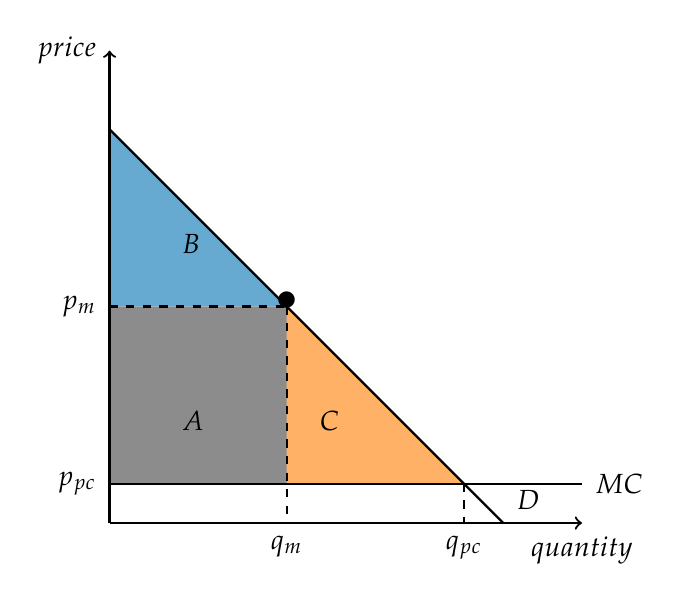
\begin{tikzpicture}[scale=0.5]
					\fill [darkgray!60] (0,1) -- (0,5.5) -- (4.5,5.5) -- (5.5,1) -- cycle;
					\fill [blue!60] (0,5.5) -- (4.5,5.5) -- (0,10) -- cycle;
					\fill [orange!60] (4.5,1) -- (4.5,5.5) -- (9,1) -- cycle;
					
					%y axis.....................
					\draw [->] (0,0) to (0,12) node [left] {$price$};
					
					%x axis......................
					\draw [->] (0,0) to (12,0) node [below] {$quantity$};
					
					% D curve...................
					\draw [thick] (0,10)  to  (10,0)  node [above right] {$D$};
					
					% MR curve....................
					%\draw [thick] (0,10) to (5,0);
					%\node [above right] at (4.5,-0.1) {$MR$};
					
					% MC=S curve...................
					\draw [thick] (0,1)  to  (12,1)  node [right] {$MC$};
					
					% dashed lines to equilibrium.............
					\draw [dashed] (0,5.5) node [left] {$p_m$} to (4.55,5.5); 
					\draw [dashed] (4.5,5.5) to (4.5,0) node [below] {$q_m$};
					
					% dashed lines to new equilibrium.........
					\draw [dashed] (0,1) node [left] {$p_{pc}$} to (9,1); 
					\draw [dashed] (9,1) to (9,0) node [below] {$q_{pc}$};
					
					% equilibrium points.......................
					\node [black] at (4.5,5.25) {\LARGE \textbullet};
					
					% labels..............................
					%\node [black, above right] at (4.5,5.5) {Monopolist's price/quantity.};
					\node [above right] at (1.5,6.5) {$B$};
					\node [above right] at (5,2) {$C$};
					\node [above right] at (1.5,2) {$A$};
				\end{tikzpicture}
			\end{figure}
		\end{column}
		\begin{column}{0.5\textwidth}
			\begin{wideitemize}
				\item We still need to optimally choose the variable part $p$.
				\item In the previous slide we saw that optimally choosing the fixed part $f$ results in the total profit = A + B.
				\item So, let's choose $p$ to make the area A + B as big as possible.
				\item This happens at $p=p_{pc}$ i.e. the perfect competition price.
			\end{wideitemize}
		\end{column}
	\end{columns}
\end{frame}

\begin{frame}{Non-linear pricing: how should the seller choose $f$ and $p$?}
	\begin{wideitemize}
	\item The \textbf{optimal two-part tariff} (with identical consumers) is:
			\item Set $p=p_{pc}$ (the perfect competition price)
			\item Set $f=CS(p_{pc})= \text{A + B + C}$ (i.e. consumer surplus under perfect competition)
			\item Note: areas A, B, C displayed on the previous slide
	\end{wideitemize}
\end{frame}

\begin{frame}{Non-linear pricing: efficiency and equity}
		\begin{wideitemize}
			\item Who were the winners and losers from moving from uniform pricing (i.e. the monopoly price) to a two-part tariff? \pause
			\begin{wideitemize}
				\item \textbf{Winner:} the sellers; profits increased from $A$ to $A+B+C$.
				\item \textbf{Loser:} consumers; consumer surplus decreased from $B$ to $0$.
			\end{wideitemize}
			\item Overall, the two-part tariff is more \textbf{efficient}. 
			\begin{wideitemize}
				\item Total surplus increases from $A+B$ to $A+B+C$. In fact, it completely eliminated all of the (inefficient) dead-weight-loss of the monopolist (area B).
			\end{wideitemize}
			\item However, this came at the cost of \textbf{equity}: consumer surplus was reduced to 0.
		\end{wideitemize}
\end{frame}

\begin{frame}{Non-linear pricing: example on p138}
	\begin{wideitemize}
		\item \textbf{Example:}
		\item Demand for each individual is given by: $q=15-2.5p$
		\item $MC=0$
		\item \textbf{Questions:}
		\item What is the optimal price and profit if the seller can only charge a per-unit price?
		\item What is the optimal two-part tariff?
	\end{wideitemize}
\end{frame}

\begin{frame}{Non-linear pricing: example on p138}
	\begin{wideitemize}
		\item \textbf{Question:} What is the optimal price and profit if the seller can only charge a per-unit price?
		\item \textbf{Solution:}
		\begin{wideitemize}
			\item Rearrange demand in terms of price: $p=6-q/2.5$
			\item Get MR using `twice the slope' trick: $MR=6-\frac{2}{2.5}q$
			\item Set MR=MC and solve for optimal $q$:  $6-\frac{2}{2.5}q=0$, so $q=7.5$
			\item Get price from demand: $p=6-7.5/2.5=3$.
			\item Profit=$3 \time 7.5=22.5$		
		\end{wideitemize}
	\end{wideitemize}
\end{frame}

\begin{frame}{Non-linear pricing: example on p138}
	\begin{wideitemize}
		\item \textbf{Question:} What is the optimal two-part tariff?
		\item \textbf{Solution:}
		\begin{wideitemize}
			\item Charge a price equal to marginal cost: $p=0$.
			\item Set a fixed fee equal to consumer surplus at $p=0$.
			\item This is: $f=\frac{1}{2} (15 \times 6) = 45$ (i.e. CS is the area under the demand curve and above MC)
			\item Profit per consumer is now \$45, double the profit under per-unit pricing.
		\end{wideitemize}
	\end{wideitemize}
\end{frame}

\begin{frame}{Non-linear pricing: case with heterogeneous consumers}
	\begin{wideitemize}
		\item This case is also considered in the textbook, but we will not consider it in this class.
	\end{wideitemize}
\end{frame}

\begin{frame}{Plan}
	\begin{wideenumerate}
		\item Non-linear pricing
		\item \textbf{Should price discrimination be legal?}
	\end{wideenumerate}
\end{frame}

\begin{frame}{Should price discrimination be legal?}
	\begin{columns}
		\begin{column}{0.4\textwidth}
			\begin{figure}
				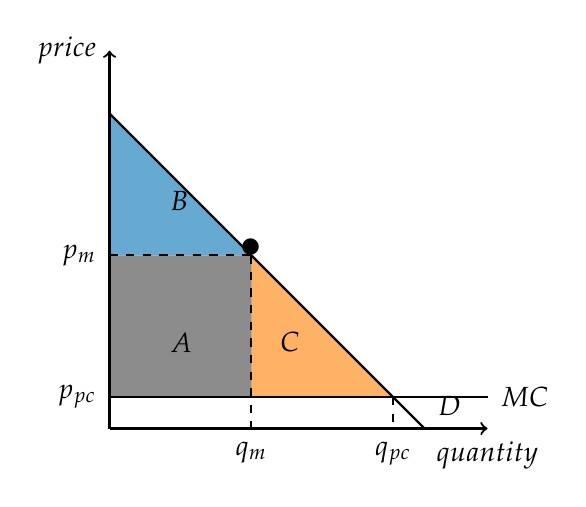
\begin{tikzpicture}[scale=0.4]
					\fill [darkgray!60] (0,1) -- (0,5.5) -- (4.5,5.5) -- (5.5,1) -- cycle;
					\fill [blue!60] (0,5.5) -- (4.5,5.5) -- (0,10) -- cycle;
					\fill [orange!60] (4.5,1) -- (4.5,5.5) -- (9,1) -- cycle;
					
					%y axis.....................
					\draw [->] (0,0) to (0,12) node [left] {$price$};
					
					%x axis......................
					\draw [->] (0,0) to (12,0) node [below] {$quantity$};
					
					% D curve...................
					\draw [thick] (0,10)  to  (10,0)  node [above right] {$D$};
					
					% MR curve....................
					%\draw [thick] (0,10) to (5,0);
					%\node [above right] at (4.5,-0.1) {$MR$};
					
					% MC=S curve...................
					\draw [thick] (0,1)  to  (12,1)  node [right] {$MC$};
					
					% dashed lines to equilibrium.............
					\draw [dashed] (0,5.5) node [left] {$p_m$} to (4.55,5.5); 
					\draw [dashed] (4.5,5.5) to (4.5,0) node [below] {$q_m$};
					
					% dashed lines to new equilibrium.........
					\draw [dashed] (0,1) node [left] {$p_{pc}$} to (9,1); 
					\draw [dashed] (9,1) to (9,0) node [below] {$q_{pc}$};
					
					% equilibrium points.......................
					\node [black] at (4.5,5.25) {\LARGE \textbullet};
					
					% labels..............................
					%\node [black, above right] at (4.5,5.5) {Monopolist's price/quantity.};
					\node [above right] at (1.5,6.5) {$B$};
					\node [above right] at (5,2) {$C$};
					\node [above right] at (1.5,2) {$A$};
				\end{tikzpicture}
			\end{figure}
		\end{column}
		\begin{column}{0.6\textwidth}
\begin{wideitemize}
	\item The non-linear pricing figure from the previous section also depicts the welfare effects of moving from uniform pricing to perfect price discrimination.
	\pause
	\item Allowing price discrimination typically:
	\begin{wideitemize}
		\item Increases total surplus ($A+B \rightarrow A+B+C$)
		\item Reduces consumer surplus ($B \rightarrow 0$)
		\begin{wideitemize}
			\item Note: it is possible to construct examples where consumers to be better off under price discrimination, but in most of the cases we will see they are worse off.
		\end{wideitemize}
		\item Results in more consumers being served ($q_m \rightarrow q_{pc}$)
	\end{wideitemize}
\end{wideitemize}
		\end{column}
	\end{columns}
\end{frame}

\begin{frame}{Should price discrimination be legal?}
	\begin{wideitemize}
		\item Whether to allow price discrimination often comes down to an \textbf{equity-efficiency tradeoff}. \pause
		\begin{wideitemize}
			\vspace{11pt}
			\item By \textit{efficiency} I am referring to the \underline{reduction in dead-weight-loss} (or, equivalently, the increase in total surplus).
			\item By \textit{equity} I am referring to the typical \underline{reduction in consumer surplus} from price discrimination (although, as mentioned in the previous slide, sometimes price discrimination will result in an increase in consumer surplus and so there will be no equity-efficiency tradeoff).
			\item Policymakers may still want to prevent pricing strategies that are efficient for equity reasons. 
		\end{wideitemize}
	\end{wideitemize}
		\begin{wideitemize}
						\vspace{11pt}
			\item Ultimately an empirical question about whether there is an \textbf{equity-efficiency tradeoff} (and where there is this tradeoff, it's up to society how we want to trade off these two competing objectives).
		\end{wideitemize}
\end{frame}

\begin{frame}{Case study: net neutrality}
	\begin{wideitemize}
		\item ISP (internet service providers) own fiber optic connections.
		\item Should they be allowed to charge different prices for different uses?
		\item Net neutrality: no price discrimination (all data has the same price) 
		\item Can you explain what the equity-efficiency tradeoff might be here? \pause
		\item Efficiency:  price discrimination may allow for a more efficient allocation of limited bandwidth (e.g. ensuring bandwidth for an important Zoom call vs watching TV)
		\item Equity:  may place some forms of content at a competitive disadvantage (e.g. how will Wikipedia pay? What about small companies?) - Netflix historically was pro-net-neutrality
	\end{wideitemize}
\end{frame}

\begin{frame}{Other issues}
	\begin{wideitemize}
		\item There are many other adjacent public policy issues to price-discrimination that are becoming increasingly more important
		\item E.g. price discrimination requires data on consumer elasticities - what is the value of this data and do consumers have a right to privacy?
		%\item GDPR (General Data Protection Regulation) in the EU: 
	\end{wideitemize}
\end{frame}

\begin{frame}{Summary of key points*}
	\vspace{11pt}
	\begin{wideitemize}
		\item Know that non-linear pricing is a pricing strategy where prices change with the quantity demanded.
		\item Know how to compute the optimal two-part tariff for homogeneous consumers (and the corresponding effects of a two-part tariff on profits, consumer surplus, etc)
		%\item Understand that the optimal two-part tariff for heterogeneous consumers involves a \textit{quantity discount} for price-discrimination by self-selection.
		\item Know that price discrimination often involves an equity-efficiency tradeoff for policymakers.
	\end{wideitemize}
	\vspace{30pt}
	*To clarify, all the material in the slides, problem sets, etc is assessable unless stated otherwise, but I hope this summary might be a useful place to start when studying the material.
\end{frame}

\begin{frame}{Ex. 6.12. RawDeal}
	\begin{wideitemize}
		\item Sushi bar. MC=0.1, demand (for each consumer) is $q=20-10p$.
		\item \textbf{Questions:}
		\item What is the optimal price per sushi unit?
		\item Consider an all-you-can-eat policy. What is the optimal price per consumer? What is the profit vs pricing per unit?
		\item What is the optimal two-part tariff for sushi (i.e. fee at the door plus a price per sushi piece)?
	\end{wideitemize}
\end{frame}

\begin{frame}{Ex. 6.12. RawDeal}
	\begin{wideitemize}
		\item Sushi bar. MC=0.1, demand (for each consumer) is $q=20-10p$.
		\item \textbf{Questions:}
		\item What is the optimal price per sushi unit? 
		\item A: p=1.05, (profit = 9.025)
		\item Consider an all-you-can-eat policy. What is the optimal price per consumer? What is the profit vs pricing per unit? 
		\item A: f=20, profit=18 (higher than before)
		\item What is the optimal two-part tariff for sushi (i.e. fee at the door plus a price per sushi piece)? 
		\item A: p=0.1, f=18.05
	\end{wideitemize}
\end{frame}

\end{document}